%%%%%%%%%%%%%%%%%%%%%%%%%%%%%%%%%%%%%%%%%
% Beamer Presentation
% LaTeX Template
% Version 1.0 (10/11/12)
%
% This template has been downloaded from:
% http://www.LaTeXTemplates.com
%
% License:
% CC BY-NC-SA 3.0 (http://creativecommons.org/licenses/by-nc-sa/3.0/)
%
%%%%%%%%%%%%%%%%%%%%%%%%%%%%%%%%%%%%%%%%%

%----------------------------------------------------------------------------------------
%	PACKAGES AND THEMES
%----------------------------------------------------------------------------------------

\documentclass{beamer}
\usepackage[utf8]{inputenc}
\usepackage[francais]{babel}

\mode<presentation> {

% The Beamer class comes with a number of default slide themes
% which change the colors and layouts of slides. Below this is a list
% of all the themes, uncomment each in turn to see what they look like.

%\usetheme{default}
%\usetheme{AnnArbor}
%\usetheme{Antibes}
%\usetheme{Bergen}
%\usetheme{Berkeley}
%\usetheme{Berlin}
%\usetheme{Boadilla}
%\usetheme{CambridgeUS}
%\usetheme{Copenhagen}
%\usetheme{Darmstadt}
%\usetheme{Dresden}
%\usetheme{Frankfurt}
%\usetheme{Goettingen}
%\usetheme{Hannover}
%\usetheme{Ilmenau}
%\usetheme{JuanLesPins}
%\usetheme{Luebeck}
\usetheme{Madrid}
%\usetheme{Malmoe}
%\usetheme{Marburg}
%\usetheme{Montpellier}
%\usetheme{PaloAlto}
%\usetheme{Pittsburgh}
%\usetheme{Rochester}
%\usetheme{Singapore}
%\usetheme{Szeged}
%\usetheme{Warsaw}

% As well as themes, the Beamer class has a number of color themes
% for any slide theme. Uncomment each of these in turn to see how it
% changes the colors of your current slide theme.

%\usecolortheme{albatross}
%\usecolortheme{beaver}
%\usecolortheme{beetle}
%\usecolortheme{crane}
%\usecolortheme{dolphin}
%\usecolortheme{dove}
%\usecolortheme{fly}
%\usecolortheme{lily}
%\usecolortheme{orchid}
%\usecolortheme{rose}
%\usecolortheme{seagull}
%\usecolortheme{seahorse}
%\usecolortheme{whale}
\usecolortheme{wolverine}

%\setbeamertemplate{footline} % To remove the footer line in all slides uncomment this line
\setbeamertemplate{footline}[page number] % To replace the footer line in all slides with a simple slide count uncomment this line

\setbeamertemplate{navigation symbols}{} % To remove the navigation symbols from the bottom of all slides uncomment this line
}

\usepackage{graphicx} % Allows including images
\usepackage{booktabs} % Allows the use of \toprule, \midrule and \bottomrule in tables

%----------------------------------------------------------------------------------------
%	TITLE PAGE
%----------------------------------------------------------------------------------------

\title[AlgAv]{Algorithmique Avancée} % The short title appears at the bottom of every slide, the full title is only on the title page

\author{Maxime Bittan - Redha Gouicem} % Your name
\date{\today} % Date, can be changed to a custom date

\begin{document}

\begin{frame}
\titlepage % Print the title page as the first slide
\end{frame}

%----------------------------------------------------------------------------------------
%	PRESENTATION SLIDES
%----------------------------------------------------------------------------------------

%------------------------------------------------
\section{Introduction} % Sections can be created in order to organize your presentation into discrete blocks, all sections and subsections are automatically printed in the table of contents as an overview of the talk
%------------------------------------------------

\begin{frame}
\frametitle{Introduction}
Comparaison de 2 types de tries :
\begin{itemize}
  \item les arbres (ou tries) de la Briandais
  \item les tries hybrides
\end{itemize}
\end{frame}

%------------------------------------------------

\begin{frame}
\frametitle{Arbres de la Briandais}
\begin{columns}[c] % The "c" option specifies centered vertical alignment while the "t" option is used for top vertical alignment

\column{.6\textwidth} % Left column and width
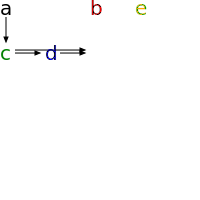
\includegraphics{figures/briandais_test.pdf}

\column{.3\textwidth} % Right column and width
%\begin{verbatim}
struct \{\\
   $\;$char clé;\\
   $\;$briandais* frere;\\
   $\;$briandais* fils;\\
   $\;$int cpt;\\
\} briandais;
%\end{verbatim}

\end{columns}
\end{frame}

%------------------------------------------------

\begin{frame}
\frametitle{Tries Hybrides}
\begin{columns}[c] % The "c" option specifies centered vertical alignment while the "t" option is used for top vertical alignment

\column{.6\textwidth} % Left column and width
\includegraphics{figures/graph_template.pdf}

\column{.35\textwidth} % Right column and width
%\begin{verbatim}
struct \{\\
   $\;$char clé;\\
   $\;$trieHybride* inferieur;\\
   $\;$trieHybride* egal;\\
   $\;$trieHybride* superieur;\\
   $\;$char fin;\\
\} trieHybride;
%\end{verbatim}

\end{columns}
\end{frame}

%------------------------------------------------
\section{Benchmarks}
%------------------------------------------------

\begin{frame}
\frametitle{Performances}
\begin{table}
\begin{tabular}{|l|l|l|}
\toprule
\textbf{Opérations} & \textbf{Briandais} & \textbf{Trie Hybride}\\
\midrule
Construire Shakespeare & 3,310641 s & 3,128169 s \\
Construire Shakespeare MT & 1,508106 s & 1,549025 s \\
Suppression & 0,126963 s & 0,115175 s \\
Recherche & 0,216970 s & 0,199453 s \\
Compter mots & 0,004294 s & 0,003283 s \\
Occupation mémoire & 2.539.008 B & 1.805.664 B \\
\bottomrule
\end{tabular}
\end{table}
\end{frame}

%------------------------------------------------

\begin{frame}
\Huge{\centerline{Merci pour votre attention !}}
\end{frame}

%----------------------------------------------------------------------------------------

\end{document}
